\chapter{Exposé: A Tree Pattern Function in Mathematica}
\label{app:Expose}

% Soure Code provision method

An exposé of the programming paradigms highlighted in Chapter \ref{cha:Theory} is included with this thesis work: It was produced as part of the companion seminar class, "Wissenschaftliches Arbeiten," i.e. Scientific Research and Writing, and serves to deliver some additional Theory about programming in WL, separately from the project focus of the main work. The author hopes this aids the interested reader and would like to point out that the document is interesting formally in that it was produced inside a Mathematica notebook, so that the cells containing text and executable WL code are of equal order inside an overall WL notebook expression, as outlined in \ref{cha:Introduction}, concerning WL expressions as document representation: as opposed to this project's \LaTeX transformation, or the native transformation also referenced in \ref{cha:Introduction}, this format represents another way, the non-\LaTeX, Mathematica-native PDF-export, for making available WL notebook content.

% Sample Document to include with thesis

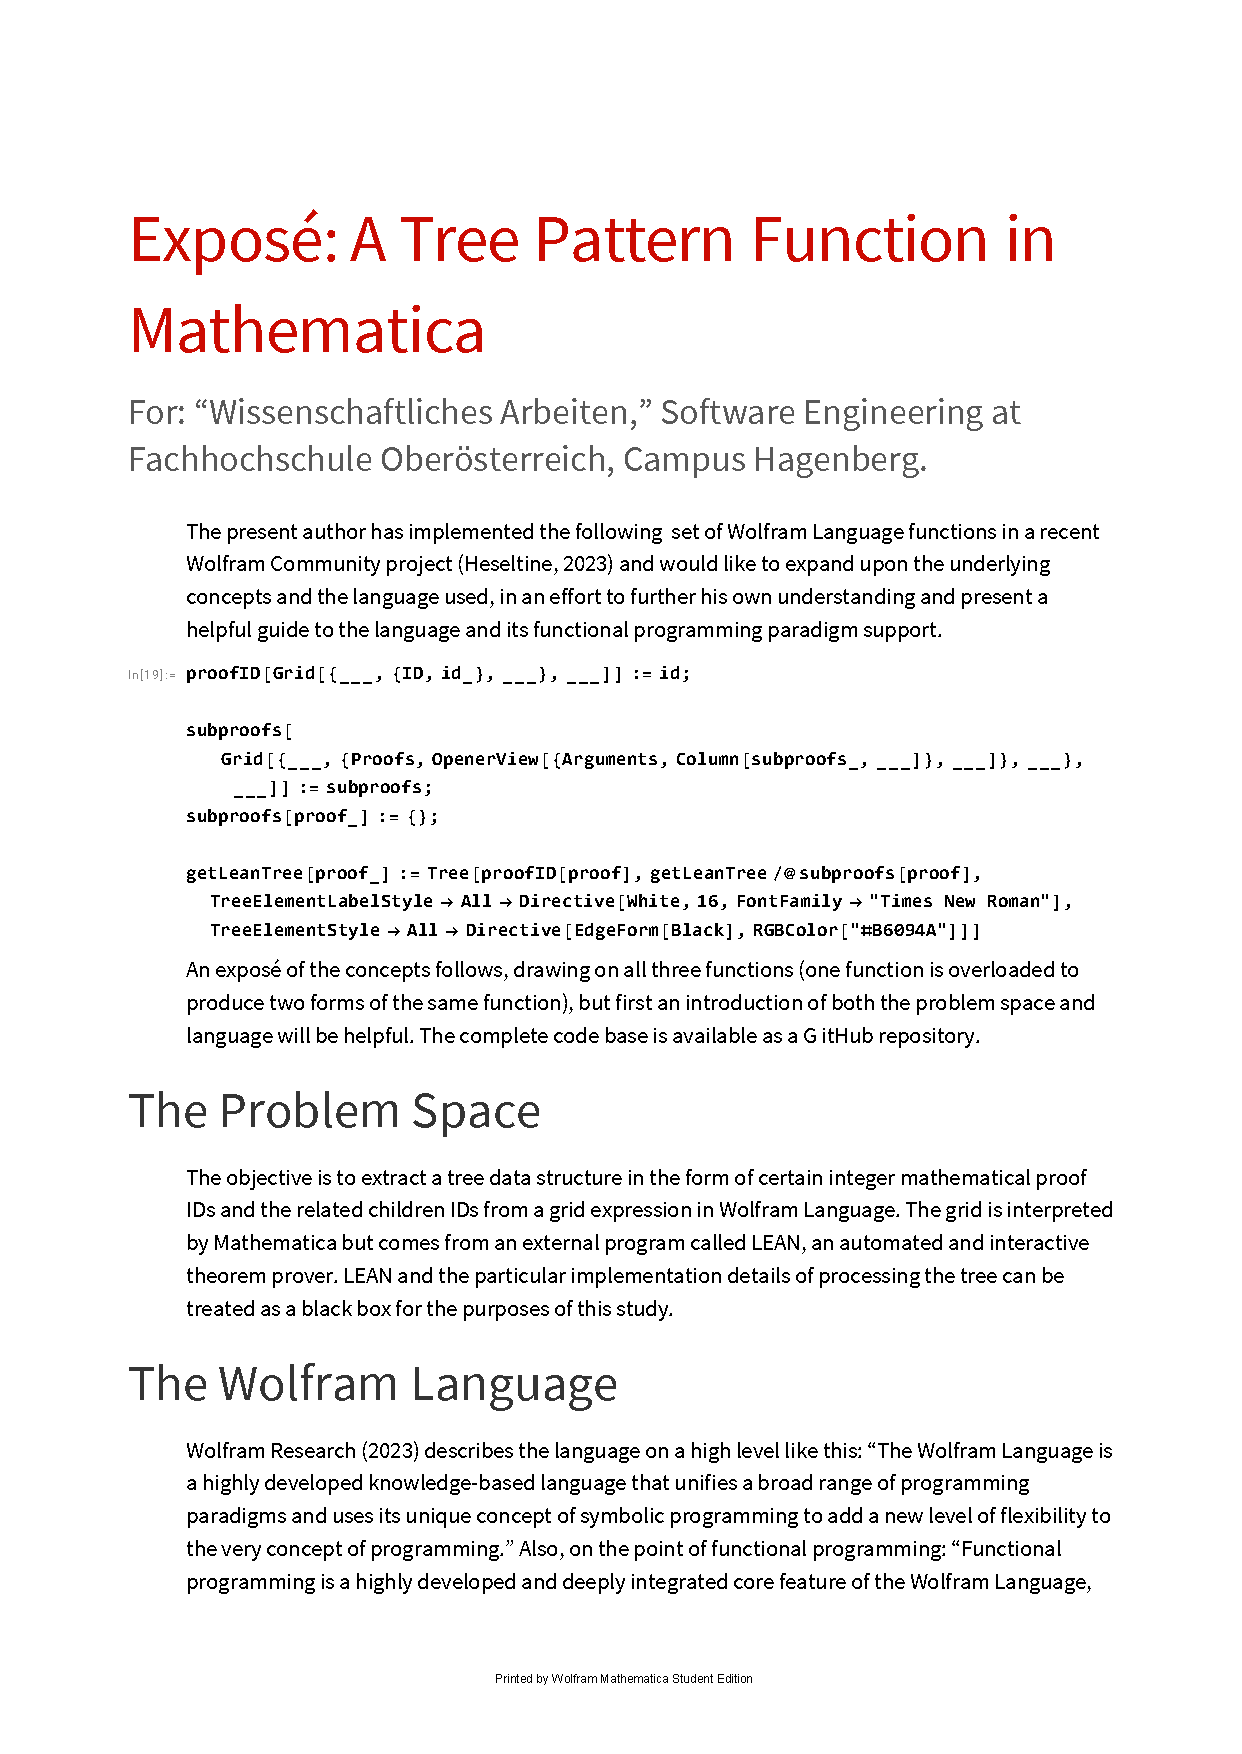
\includepdf[pages=-,frame,scale=0.95,pagecommand={}]{furtherpdfincludes/expose-tree-pattern-function-native-export.pdf}